\documentclass[12pt]{article}
\usepackage{amsmath}
\usepackage{amsthm}
\usepackage{graphicx,psfrag,epsf}
\usepackage{enumerate}
\usepackage{natbib}
\usepackage{url} % not crucial - just used below for the URL
\usepackage{color}
\usepackage{mathtools}

%\pdfminorversion=4
% NOTE: To produce blinded version, replace "0" with "1" below.
\newcommand{\blind}{0}

% DON'T change margins - should be 1 inch all around.
\addtolength{\oddsidemargin}{-.5in}%
\addtolength{\evensidemargin}{-.5in}%
\addtolength{\textwidth}{1in}%
\addtolength{\textheight}{1.3in}%
\addtolength{\topmargin}{-.8in}%


%%%% Packages and definitions
\usepackage{amssymb}

\usepackage{xr}

\usepackage[top=0.85in,left=1.0in,right=1.0in,footskip=0.75in]{geometry}

% Use adjustwidth environment to exceed column width (see example table in text)
\usepackage{changepage}

% Use Unicode characters when possible
\usepackage[utf8]{inputenc}

% textcomp package and marvosym package for additional characters
\usepackage{textcomp,marvosym}

\usepackage[ruled]{algorithm}
\usepackage{algorithmic}

% cite package, to clean up citations in the main text. Do not remove.
\usepackage{cite}

% Use nameref to cite supporting information files (see Supporting Information section for more info)
\usepackage{nameref,hyperref}

%\usepackage{amsthm}

% ligatures disabled
\usepackage{microtype}
\DisableLigatures[f]{encoding = *, family = * }

% for the beautiful checkmarks
\usepackage{pifont}

\newtheorem{theorem}{Theorem}
\newtheorem{corollary}{Corollary}
\newtheorem{lemma}{Lemma}
\newtheorem{definition}{Definition}
\newtheorem{condition}{Condition}

\DeclareMathOperator*{\argmin}{arg\,min}


\begin{document}

\def\spacingset#1{\renewcommand{\baselinestretch}%
{#1}\small\normalsize} \spacingset{1}


%%%%%%%%%%%%%%%%%%%%%%%%%%%%%%%%%%%%%%%%%%%%%%%%%%%%%%%%%%%%%%%%%%%%%%%%%%%%%%

\if0\blind
{
  \title{\bf Oracle inequalities for tuning hyperparameters via validation sets with applications to penalized regression}
  \author{Jean Feng\thanks{
    Jean Feng was supported by NIH grants ???. % DP5OD019820 and T32CA206089.
    Noah Simon was supported by NIH grant DP5OD019820.
    The content is solely the responsibility of the authors and does not necessarily represent the official views of the National Institutes of Health.}\\
    Department of Biostatistics, University of Washington\\
    and \\
    Noah Simon \\
    Department of Biostatistics, University of Washington}
  \maketitle
} \fi

\if1\blind
{
  \bigskip
  \bigskip
  \bigskip
  \begin{center}
    {\LARGE\bf title goes here}
\end{center}
  \medskip
} \fi

\bigskip
\begin{abstract}

\textcolor{red}{You say ``model error'' a lot. This isn't really a precise term. Be more precise.} In the regression setting, given a set of hyper-parameters, a model-estimation procedure constructs a model from training data. The optimal hyperparameters, that minimize generalization error of the model, are usually unknown. In practice they are often estimated using split-sample validation. Up to now, there is an open question regarding how the generalization error of the selected model grows with the number of hyperparameters to be estimated. To answer this question, we establish finite-sample oracle inequalities for selection based on a single training/test split and based on cross-validation. We show that if the model-estimation procedures are smoothly parameterized by the hyperparameters, the error incurred from tuning hyperparameters shrinks at nearly a parametric rate. Hence for semi- and non-parametric model-estimation procedures, for a fixed number of hyperparameters, this additional error is negligible. For parametric model-estimation procedures, adding a hyperparameter is roughly equivalent to adding a parameter to the model itself. In addition, we specialize these ideas for penalized regression problems with multiple penalty parameters. We establish that the fitted models are Lipschitz in the penalty parameters and thus our oracle inequalities apply. This result encourages development of regularization methods with many penalty parameters.
\end{abstract}

\noindent%
{\it Keywords:}  Hyperparameter selection, Cross-validation, Regularization, Regression
\vfill

\newpage
\spacingset{1.45}
\section{Introduction}

Per the usual regression framework, suppose we observe response $y \in \mathbb{R}$ and predictors $\boldsymbol {x} \in \mathbb{R}^p$. Suppose $y$ is generated by a true model $g^*$ plus random error $\epsilon$ with $\operatorname{E}\left[\epsilon\right] = 0$, as follows
\begin{equation}
\label{true_model}
y = g^*(\boldsymbol x) + \epsilon
\end{equation}
Our goal is to estimate $g^*$.

Many model-estimation procedures can be formulated as selecting a model from some function class $\mathcal{G}$ given training data $T$ and $J$-dimensional hyperparameter vector $\boldsymbol{\lambda}$. For example, in penalized regression problems, the fitted model can be expressed as the minimizer of the penalized training criterion
\begin{equation}
\label{eq:intro_pen_reg}
\hat{g}(\boldsymbol \lambda | T) = \argmin_{g\in \mathcal{G}} \sum_{(x_i, y_i) \in T} \left (y_i -  g(x_i) \right )^2 + \sum_{j=1}^J \lambda_j P_j(g)
\end{equation}
where $P_j$ are penalty functions and $\lambda_j$ are penalty parameters. As suggested by the notation in \eqref{eq:intro_pen_reg}, the penalty parameters are the hyperparameters in this model-estimation procedure.

Given a set of possible hyperparameters $\Lambda$, for a given training dataset $T$ and norm $\|\cdot\|$, there is some oracle hyperparameter $\tilde{\boldsymbol{\lambda}} \in \Lambda$ that minimizes the difference between the fitted model and the true model:
\[
\tilde{\boldsymbol{\lambda}} = \argmin_{\lambda \in \Lambda} \left\|g^{*} - \hat{g}\left(\boldsymbol{\lambda|}T\right)\right\|^2
\]
$\tilde{\boldsymbol{\lambda}}$ is unknown and often estimated using a single training/validation split or cross-validation. The basic idea is to fit models on a random partition of the observed data and evaluate their error on the remaining data. The final hyperparameters $\hat{\boldsymbol{\lambda}}$ are the minimizer of the error on this validation set. For a more complete review of cross-validation, refer to \citet{arlot2010survey}.

The performance of split-sample validation procedures is typically characterized by an oracle inequality that bounds the generalization error of the expected model selected from the validation set procedure. For $\Lambda$ that are finite, oracle inequalities have been established for a single training/validation split \citet{gyorfi2006distribution} and a general cross-validation framework \citep{van2003unified, van2004asymptotic}. To handle continuous $\Lambda$, one can use entropy-based approaches \citep{lecue2012oracle}. 

The goal of this paper is to characterize the performance of models when the hyperparameters must be tuned by some split-sample validation procedure. We are particularly interested in an open question raised in \citet{bengio2000gradient} (and others): what is the ``amount of overfitting... when too many hyperparameters are optimized''? To do this, we establish finite-sample oracle inequalities of the form
\begin{equation}
\label{thrm:intro_oracle_ineq}
\left \| g^* - \hat{g}\left (\hat{\boldsymbol{\lambda}}, T \right ) \right \|^2
\le
(1+a)
\underbrace{\inf_{\lambda \in \Lambda} \left \| g^* - \hat{g}\left (\boldsymbol{\lambda} , T \right ) \right \|^2}_{\text{Oracle error}}
+ \delta\left(J,n\right)
\end{equation}
for some norm $\| \cdot \|$ and constant $a \ge 0$; where $\delta(J,n)$ is a function of the number of parameters to tune and the number of validation samples $n$. Under the assumption that the model-estimation procedure is smoothly parameterized by the hyperparameters, we find that the contribution to $\delta$ from tuning hyperparameters is roughly a parametric rate. For parametric model-estimation procedures, the additional error from adding a hyperparameter is roughly equivalent to adding a parameter to the model itself. For semi- and non-parametric model-estimation procedures, this error is generally dominated by the oracle error and the number of hyperparameters can actually grow without affecting the asymptotic convergence rate.

In this paper, we also specialize these results to penalized regression models of the form \eqref{eq:intro_pen_reg}. We show that the fitted model is indeed smoothly parameterized by the penalty parameters so our oracle inequalities apply. Again, we find that additional penalty parameters only add a near-parametric error term, which has a negligible effect on the model error in semi- and non-parametric settings. This result suggests that the recent interest in combining penalty functions (e.g. elastic net and sparse group lasso \citep{zou2003regression, simon2013sparse}) may have artificially restricted themselves to two-way combinations. Adding more penalties may lead to better models.

We did not find any theoretical results addressing the relationship betwen the number of hyperparameters and model error. Most oracle inequalities only consider one-dimensional hyperparameters \citep{van2003unified, van2004asymptotic, gyorfi2006distribution}. Within the context of penalized regression problems, the oracle inequalities are also only for the case of a single penalty parameter \citep{golub1979generalized, chetverikov2016cross, chatterjee2015prediction}. Only \citet{lecue2012oracle} has a result that is relevant to answering our question of interest. We will use his framework to address the question of cross-validation for multiple hyperparameters. A potential reason for this dearth of literature is that, historically, tuning multiple hyperparameters has been computationally difficult. However, there have been many proposals recently for overcoming this computational hurdle \citep{bengio2000gradient, foo2008efficient, snoek2012practical}.

Section \ref{sec:main_results} presents oracle inequalities for model-estimation procedures that are smoothly parameterized by the hyperparameters. These results answer our question regarding how the number of hyperparameters affects the model error.
Section \ref{sec:examples} applies these results to penalized regression models.
Section \ref{sec:simulations} provides a simulation study to support our theoretical results.
Section \ref{sec:discussion} discusses our findings and potential future work.
Section \ref{sec:proofs} presents oracle inequalities for general model-estimation procedures and proofs for all the results.


\section{Main Result} \label{sec:main_results}

In this section, we establish oracle inequalities for the model error from tuning hyperparameters by a single training/validation split and cross-validation.
We first introduce some notation and formalize the model-estimation procedure. 

Let $D^{(n)}$ denote a dataset with $n$ samples from the model \eqref{true_model}. The model-estimation procedure accepts some hyperparameter of dimension $J$ and training data of size $n_T$ to output a fitted model from some model class $\mathcal{G}$. This can be formulated as an operator $\hat{g}^{(n_T)}(\cdot | D^{(n_T)})$ that maps a hyperparameter vector $\boldsymbol{\lambda}$ from some set $\Lambda \subseteq \mathbb{R}^J$ to a function in $\mathcal{G}$. 

In this section, we focus on model-estimation procedures that are Lipschitz.
\begin{definition}
	\label{def:smooth_funcs}
	Let $\mathcal{F}$ be a function class. Let $\Lambda \subseteq \mathbb{R}^J$.
	The operator $\hat{f}: \Lambda \mapsto \mathcal{F}$ is $C$-Lipschitz in $\boldsymbol{\lambda}$ with respect to norm $\| \cdot \|$ over $\Lambda$ if
	\begin{equation}
	\left \| \hat{f}(\boldsymbol \lambda) - \hat{f}(\boldsymbol \lambda ') \right \|
	\le
	C \| \boldsymbol \lambda - \boldsymbol \lambda' \|_2 
	\quad
	\forall \boldsymbol \lambda,\boldsymbol \lambda' \in \Lambda
	\label{eq:smooth_funcs}
	\end{equation}
\end{definition}
We hypothesize that many model-estimation procedures satisfy this Lipschitz assumption since it ensures that the procedure is well-behaved. Section \ref{sec:examples} shows that penalized regression models indeed satisfy this assumption. The following results (from Sections~\ref{sec:single},\ref{sec:cv}) show that the contribution to the error from tuning multiple hyperparameters for such procedures is roughly parametric. Hence for semi- or non-parametric model-estimation procedures, the error from tuning a fixed number of hyperparameters is negligible. In fact, we specify a bound on the rate at which the number of hyperparameters can grow in such problems without asymptotically increasing the generalization error from the oracle model.

\subsection{A single Training/Validation Split}\label{sec:single}

For a single training/validation split, the dataset $D^{(n)}$ is randomly partitioned into a training set $T = (X_T, Y_T)$ and validation set $V = (X_V, Y_V)$ with $n_T$ and $n_V$ observations, respectively. The selected hyperparameter $\hat{\boldsymbol{\lambda}}$ is the minimizer of the validation loss
\begin{equation}
\label{eq:train_val_lambda}
\hat{\boldsymbol \lambda} = \argmin_{\boldsymbol{\lambda} \in\Lambda} \frac{1}{2} \left \| y-\hat{g}^{(n_T)}( \boldsymbol \lambda | D_T^{(n_T)}) \right \|_{V}^{2}
\end{equation}
where $\| h \|_{V}=\frac{1}{n_V}\sum_{i\in V} h^2(x_i)$ for any function $h$. 

We now present a finite-sample oracle inequality for the single training/validation split assuming the model-estimation procedure is Lipschitz. Our oracle inequality is sharp, i.e. $a=0$ in \eqref{thrm:intro_oracle_ineq}, unlike most other work \citep{gyorfi2006distribution, lecue2012oracle, van2003unified}. Note that the result below is a special case of our Theorem \ref{thrm:train_val_complicated} in Appendix \ref{appendix:train_val}, which applies to general model-estimation procedures.
\begin{theorem}
\label{thrm:train_val}
Let $\Lambda=[\lambda_{\min},\lambda_{\max}]^{J}$ where $0 < \lambda_{\min} < \lambda_{\max}$. Suppose independent random variables $\epsilon_1, ... \epsilon_n$ have expectation zero and are uniformly sub-Gaussian with parameter $b > 0$:
$$
\max_{i=1,...,n} \mathbb{E} e^{t \epsilon_i} \le e^{b^2t^2/2} \quad \forall t \in \mathbb{R}
$$
Suppose there is a constant $C_\Lambda \ge 32e/(n \lambda_{\max})$ such that $\hat g^{(n_T)}(\boldsymbol{\lambda} |D^{(n_T)})$ is $C_\Lambda$-Lipschitz with respect to $\| \cdot \|_V$ over $\Lambda$.

Let 
\begin{equation}
\tilde{\boldsymbol \lambda} = \argmin_{\lambda \in \Lambda} \left \| g^*-\hat{g}^{(n_T)}( \boldsymbol{\lambda} | T) \right \|_{V}^{2}
\label{eq:tilde_lambda_def}
\end{equation}

Then there is a constant $c>0$ only depending on $b$ such that for all $\delta$ satisfying
\begin{equation}
\delta^{2}
\ge
c \left ( 
\frac{J\log (n C_\Lambda\lambda_{\max})}{n_{V}}
\vee 
\sqrt{\frac{J \log (n C_\Lambda \lambda_{\max})}{n_{V}}\left\Vert g^* - \hat{g}^{(n_T)}( \tilde{\boldsymbol{\lambda}} | T)\right\Vert_{V}^2}
\right )
\label{thrm:train_val_delta}
\end{equation}
we have
\begin{eqnarray*}
	Pr\left(
	\left\Vert g^* - \hat{g}^{(n_T)}( \hat{\boldsymbol{\lambda}} | T) \right\Vert _{V}^2 -
	\left\Vert g^* - \hat{g}^{(n_T)}( \tilde{\boldsymbol{\lambda}} | T) \right\Vert _{V}^2
	\ge\delta^2
	\middle | 
	T, X_V
	\right )
	&\le& c\exp\left(-\frac{n_{V}\delta^{4}}{
		c^{2}
		\left\Vert g^* - \hat{g}^{(n_T)}( \tilde{\boldsymbol{\lambda}} | T) \right\Vert _{V}^2
	}\right) \\
	&& +c\exp\left(-\frac{n_{V}\delta^{2}}{c^{2}}\right) \\
\end{eqnarray*}

\end{theorem}

Theorem \ref{thrm:train_val} states that as the number of validation samples grows, the difference between the selected model error and the oracle model error shrinks at the rate of $\delta^2$ with high probability. $\delta^2$ can be thought of as the error incurred during the hyperparameter selection process. As seen in \eqref{thrm:train_val_delta}, it is the maximum of two terms: a near-parametric term and a geometric mean of the near-parametric term and the oracle error. To see this more clearly, we express Theorem \ref{thrm:train_val} using asymptotic notation.
\begin{corollary}
	\label{corr:train_val}
	Under the assumptions given in Theorem \ref{thrm:train_val}, we have
	\begin{eqnarray}
	\left\Vert g^* - \hat{g}^{(n_T)}( \hat{\boldsymbol{\lambda}} | T) \right\Vert _{V}^2 &\le& \left\Vert g^* - \hat{g}^{(n_T)}( \tilde{\boldsymbol{\lambda}} | T) \right \Vert^2_{V}\\
	&& + O_p \left(\frac{J\log (n C_\Lambda\lambda_{\max})}{n_{V}} \right) 
	\label{eq:asym_train_val_theorem1} \\
	&& + O_p \left(
	\sqrt{
		\frac{J \log (n C_\Lambda\lambda_{\max})}{n_{V}}
		\left\Vert g^* - \hat{g}^{(n_T)}( \tilde{\boldsymbol{\lambda}}| T) \right \Vert^2_{V}
	}
	\right )
	\label{eq:asym_train_val_theorem2}
	\end{eqnarray}
\end{corollary}
Hence the error of the selected model is bounded by the error of the oracle model, the near-parameteric term \eqref{eq:asym_train_val_theorem1}, and the geometric mean of the two values \eqref{eq:asym_train_val_theorem2}. We refer to \eqref{eq:asym_train_val_theorem1} as near-parametric because the error term in parametric regression models are usually $O_p(J/n)$, where $J$ is the parameter dimension and $n$ is the number of training samples. Analogously, \eqref{eq:asym_train_val_theorem1} is roughly $O_p(J/n_V)$ modulo a $\log n$ term in the numerator.

In the semi- and non-parametric regression settings, the oracle error usually shrinks at a rate of $n^{-\omega}$ where $\omega \in (0, 1)$, which means that for large $n$, the oracle error will tend to dominate both the error terms. Therefore increasing the number of hyperparameters for such problems only results in small increases in the model error/degree of overfitting. In fact, if the oracle error rate is $O_p(n^{-\omega})$, the number of hyperparameters $J$ can grow at the rate
\begin{equation}
\frac{n_{V} n^{-\omega}}{\log (n C_\Lambda\lambda_{\max})}
\end{equation}
without affecting the asymptotic convergence rate. Note that for parametric regression problems, this will not be the case. \textcolor{red}{Noah: I think the bound in (10) should give $n_vn^{-\omega/2}/\operatorname{log}(n)$ (I think that second one should be the bound?) Jean: I think you forgot that (10) has a $\sqrt{J}$, not a $J$. The growth rate of $J$ should be the same whether you use (9) or (10).}

The appearance of the parametric term \eqref{eq:asym_train_val_theorem1} suggests that we can interpret the problem of tuning hyperparameters as a parametric regression problem over a $J$-dimensional parameter space where the validation data is the training data. However, this interpretation is an oversimplification. Recall that we perform the training/validation split over the model class
\begin{equation}
\mathcal{G}(T) = \left \{ \hat{g}^{(n_T)}( {\boldsymbol{\lambda}}| T) : \boldsymbol{\lambda} \in \Lambda \right \}
\end{equation}
$\mathcal{G}(T)$ is unlikely to contain the true model $g^*$ and is biased by
\begin{equation}
\min_{\lambda \in \Lambda} \left\Vert g^* - \hat{g}^{(n_T)}( \boldsymbol{\lambda}|T) \right \Vert^2_{V}
\end{equation}
This bias term contributes to the convergence rate in the geometric mean \eqref{eq:asym_train_val_theorem2}.

\subsection{Cross-Validation}\label{sec:cv}

In this section, we give an oracle inequality for $K$-fold cross-validation. Previously, the oracle inequality was with respect to the L2 norm over the validation covariates. Now, we give our result with respect to the generalization error
\begin{equation}
\left \| g - g^* \right \|^2 = \int \left |g(x) - g^*(x) \right |^2 dx
\end{equation}

For $K$-fold cross-validation our setup is as follows. Let dataset $D^{(n)}$ be randomly partitioned into $K$ sets, which we assume to have equal size for simplicity. Partition $k$ will be denoted $D_k^{(n_V)}$ and its complement will be denoted $D_{-k}^{(n_T)} = D \setminus D_k^{(n_V)}$. We perform our model-selection procedure over $D_{-k}^{(n_T)}$ for $k=1,...,K$ and select the hyperparameter that minimizes the average validation loss
\begin{eqnarray}
\label{kfold_opt}
\hat{\boldsymbol \lambda} &=& \argmin_{\boldsymbol{\lambda} \in\Lambda} \frac{1}{2K} \sum_{k=1}^K  \left \| y-\hat{g}^{(n_T)}(\boldsymbol \lambda | D_{-k}^{(n_T)}) \right \|_{D_k^{(n_V)}}^{2}
\end{eqnarray}

In traditional cross-validation, the final model is retrained on all the data with $\hat{\boldsymbol{\lambda}}$. However, bounding the generalization error of the retrained model requires additional regularity assumptions \citep{lecue2012oracle}. We consider the ``averaged version of cross-validation'' instead
\begin{equation}
\label{thrm:avg_cv}
\bar{g}\left ( \hat{\boldsymbol \lambda} \middle | {D^{(n)}} \right ) = 
\frac{1}{K} \sum_{k=1}^K 
\hat{g}^{(n_T)} \left (\hat{\boldsymbol \lambda} \middle | D^{(n_T)}_{-k} \right )
\end{equation}

The following theorem bounds the generalization error of \eqref{thrm:avg_cv}. It is an application of Theorem 3.5 in \citet{lecue2012oracle}, which is reproduced in Theorem \ref{thrm:k_fold_complicated} for convenience.

\begin{theorem}
\label{thrm:kfold}
Let $\Lambda = [\lambda_{\min}, \lambda_{\max}]^J$. Suppose there is a $G \ge  2$ such that $\sup_{g \in \mathcal{G}} \|g\|_\infty \le G$.

Consider datasets of size $n$ where $n$ is divisible by $K$, for $K \ge 2$.
Suppose random variables $\epsilon_i$ are independent with expectation zero and are bounded $\| \epsilon_i \|_\infty \le \sigma$. Suppose there is a constant $C_\Lambda >0$ such that for any dataset $D^{(n_T)}$, $\hat g (\boldsymbol{\lambda} | D^{(n_T)})$ is $C_\Lambda$-Lipschitz with respect to $\| \cdot \|_\infty$ over $\Lambda$.

Then there are absolute constants $c_1, c_2 > 0$ such that for all $a > 0$,
\begin{eqnarray}
E_{D^{(n)}} \left \| \bar{g} ( \hat{\boldsymbol \lambda} | {D^{(n)}} ) - g^* \right \|^2 &\le&
(1+a) \min_{\boldsymbol{\lambda} \in \Lambda}  E_{D^{(n_T)}} \left \| \hat{g}^{(n_T)}(\boldsymbol \lambda | D^{(n_T)}) - g^* \right \|^2 \\
&& + c_1 \frac{(1+a)^2}{a} \frac{J}{n_V} 
\left (
G \log (GC_\Lambda \lambda_{max} ) \log n + c_2
\right )
\end{eqnarray}
\end{theorem}

As we can see, Theorems \ref{thrm:train_val} and \ref{thrm:kfold} are quite similar. The upper bounds in both theorems depend on the oracle error and a near-parametric term. For parametric model-estimation procedures, tuning hyperparameters incurs a similar cost as the model-estimation procedure itself. In semi- and non-parametric regression settings, tuning hyperparameters is a relatively ``cheap'' and incurs an error that is negligible asymptotically.

There are also some notable differences between Theorems \ref{thrm:train_val} and \ref{thrm:kfold}. The Lipschitz condition in Theorem \ref{thrm:kfold} is required to hold with respect to $\| \cdot \|_\infty$, which is stricter than that in Theorem \ref{thrm:train_val}. Also, we no longer have a sharp oracle inequality since the oracle error is scaled by $1+a$ where $a > 0$. These differences occur when we are interested in characterizing the generalization error instead.

%Finally, since the theorems in this section are finite-sample results, one could try to minimize the upper bound by increasing the number of hyperparameters or changing the ratio between the training and validation set sizes. Unfortunately, optimizing the upper bound in these oracle inequalities require knowing characteristics about the error variables. Instead one may need to rely on heuristic approaches (or even another layer of cross-validation).

\section{Penalized regression models}
\label{sec:examples}

Penalized regression is a class of model-generating procedures where hyperparameters are of particular interest. In this manuscript, we consider penalized regression procedures of the form \eqref{eq:intro_pen_reg}. Penalty functions are used to control model complexity and induce desired characteristics (e.g. smoothness or sparsity). When multiple penalty functions are used, the resulting model exhibits a combination of the desired characteristics. Hence there has been recent interest in combining penalty functions, such as the elastic net or sparse group lasso. However few popular methods use more than two penalties. This has been due to a) the concern that models may overfit the data when selection of many penalty parameters is required; and b) computational issues in optimizing multiple penalty parameters. In this section, we evaluate the validity of concern (a), using the results of Section~\ref{sec:main_results}: We see that, contrary to popular wisdom, using split-sample validation to select multiple penalty parameters should not result in overfitting (even if many parameters need to be tuned). For computational concerns (b), we refer the reader to recent papers on hyperparameter estimation \citep{bengio2000gradient, foo2008efficient, snoek2012practical}.

Recall that in our framework, the model-estimation procedure takes in penalty parameters (i.e. hyperparameters) and then finds the minimizer of the penalized training criterion \eqref{eq:intro_pen_reg}. Models are fit for penalty parameters within some set $\Lambda$. As long as we can show that the fitted models are Lipschitz in the penalty parameters over $\Lambda$, we can apply Theorems \ref{thrm:train_val} and \ref{thrm:kfold}.

Our results do not allow us to consider split-sample validation over all $\lambda\in\mathbb{R}^J_+$: generally as $\lambda_{min} \rightarrow 0$, for any finite $n$, our fitted models become very widely behaved. Instead we restrict ourselves to 
\begin{equation}
\label{thrm:lambda_range}
\Lambda = [ n^{-t_{\min}}, n^{t_{\max}}]^J
\end{equation}
for sufficiently large $t_{\min}, t_{\max} \ge 0$. This regime works well for two reasons: a) our rates depend only quite weakly on $t_{\min}$ and $t_{\max}$; and 2) generally oracle $\lambda$-values are $\sim n^{-\alpha}$ for some $\alpha \in (0,1)$ \citep{van2000empirical, van2014additive, buhlmann2011statistics}. So long as $t_{\min} > \alpha$, we will ensure that $\Lambda$ contains the optimal penalty parameters over all of $\mathbb{R}^J_+$.

If $\Lambda$ is of the form \eqref{thrm:lambda_range}, we find that the Lipschitz constant for many penalized regression examples are polynomial in $n$, such as in Sections \ref{sec:param_smooth}, \ref{sec:param_nonsmooth}, and \ref{sec:nonparam_smooth}. That is, there exist constants $C, \kappa \ge 0$ such that
\begin{equation}
\label{thrm:lipschitz_pen_reg}
\left \| \hat{g}^{(n_T)}(\boldsymbol{\lambda}|T) - \hat{g}^{(n_T)}(\boldsymbol{\lambda}'|T) \right \| \le C n^\kappa \left \| \boldsymbol{\lambda} - \boldsymbol{\lambda}' \right \| \quad \forall \boldsymbol{\lambda}, \boldsymbol{\lambda}' \in \Lambda
\end{equation}
In our examples, the Lipschitz constant is inversely proportional to $\lambda_{\min}$, so $\kappa$ grows linearly in $t_{\min}$. Assuming that \eqref{thrm:lambda_range} and \eqref{thrm:lipschitz_pen_reg} hold, we get the following oracle inequalities when tuning penalty parameters via the single training/validation split and cross-validation. 
\begin{corollary}
	 Suppose $\lambda_{\min} = n^{-t_{\min}}$ and $\lambda_{\max} = n^{t_{\max}}$ for $t_{\min}, t_{\max} \ge 0$. Let $C, \kappa  > 0$.
	 
	 \begin{enumerate}
	 	\item Single training/validation split: Suppose conditions in Theorem \ref{thrm:train_val} hold with $C_\Lambda = C n^\kappa$. Then 
		\begin{eqnarray}
		\left\Vert g^* - \hat{g}^{(n_T)}( \hat{\boldsymbol{\lambda}} | T) \right\Vert _{V}^2 &\le& \left\Vert g^* - \hat{g}^{(n_T)}( \tilde{\boldsymbol{\lambda}} | T) \right \Vert^2_{V}\\
		&& + O_p \left(\frac{J (1 + \kappa + t_{\max})\log n}{n_{V}} \right) 
		\\
		&& + O_p \left(
		\sqrt{
			\frac{J (1 + \kappa + t_{\max})\log n}{n_{V}}
			\left\Vert g^* - \hat{g}^{(n_T)}( \tilde{\boldsymbol{\lambda}}| T) \right \Vert^2_{V}
		}
		\right )
		\end{eqnarray}
	 	
	 	\item Averaged version of $K$-fold cross-validation: Suppose conditions in Theorem \ref{thrm:kfold}  hold with $C_\Lambda = C n^\kappa$. Then for sufficiently large $n$, there is an absolute constant $c_1 > 0$ such that for all $a > 0$,
	 	\begin{eqnarray}
	 	E_{D^{(n)}} \left \| \bar{g} ( \hat{\boldsymbol \lambda} | {D^{(n)}} ) - g^* \right \|^2 &\le&
	 	(1+a) \min_{\boldsymbol{\lambda} \in \Lambda}  E_{D^{(n_T)}} \left \| \hat{g}^{(n_T)}(\boldsymbol \lambda | D^{(n_T)}) - g^* \right \|^2 \\
	 	&& + c_1 \frac{(1+a)^2}{a} 
	 	\frac{J (t_{\max} + \kappa) (\log n)^2}{n_V} 
	 	\end{eqnarray}
	 \end{enumerate}
\end{corollary}
We get very similar results to those in Corollary \ref{corr:train_val} and Theorem \ref{thrm:kfold}. We still have the same near-parametric term and geometric mean in the oracle inequality for the single training/validation split and a near-parametric term in the oracle inequality for cross-validation. The near-parametric terms have the familiar $\log n$ in the numerator because the error terms are proportional to the log of the Lipschitz constant and $\lambda_{\max}$. 

Therefore we reach the same conclusion for the relationship between penalty parameters and model error. In high dimensional and non-parametric penalized regression problems satisfying \eqref{thrm:lipschitz_pen_reg}, the error from tuning penalty parameters is negligible compared to the error from solving the penalized regression problem itself.

It remains to characterize those penalized problems wherein the fitted models are Lipschitz in the penalty parameters. In this manuscript we will do an in-depth study of additive models, which have the form
\begin{equation}
g(x_1, ..., x_J)= \sum_{j=1}^J g_j(x_j)
\end{equation}
though we believe that these results hold much more generally. We first consider parametric additive models (with potentially growing numbers of parameters) fitted with smooth and non-smooth penalties and then nonparametric additive models. Results for more general penalized regression may be derived in a similar manner (note that if the fitted models are not exactly Lipschitz, one would need the more general oracle inequalities from Theorems \ref{thrm:train_val_complicated} and \ref{thrm:mitchell} instead). \textcolor{blue}{I don't think I have space for putting results for more general penalized regression problems.}

\subsection{Parametric additive models}
\label{sec:param_add_models}
\textcolor{red}{GOT TO HERE!} Parametric additive models have the form
\begin{equation}
g(\cdot | \boldsymbol{\theta}^{(1)}, ..., \boldsymbol{\theta}^{(J)}) = \sum_{j=1}^J g_j(\cdot | \boldsymbol{\theta}^{(j)})
\end{equation}
where $\boldsymbol{\theta}^{(j)} \in \mathbb{R}^{p_j}$ and $p = \sum_{j=1}^J p_j$. The number of dimensions $p_j$ is allowed to grow with $n$, as commonly done in sieve estimation. For simplicity, let the full parameter vector be denoted $\boldsymbol{\theta} = \left (\boldsymbol{\theta}^{(1)}, ..., \boldsymbol{\theta}^{(J)} \right )^\top$. Then we can write the training criterion for training data $T$ as
\begin{equation}
\label{eq:param_add}
L_T \left (\boldsymbol{\theta}, \boldsymbol{\lambda} \right) 
\coloneqq \frac{1}{2} \left  \| y -  g(\boldsymbol{\theta}) \right \|^2_T 
+ \sum_{j=1}^J \lambda_j P_j(\boldsymbol{\theta}^{(j)})
\end{equation}
Suppose the true model has parameters $\boldsymbol{\theta}^*$.

%\footnote{Many popular estimators are Lipschitz since we usually construct the model by taking a linear combination of some basis functions.}

\subsubsection{Parametric regression with smooth penalties}
\label{sec:param_smooth}
We begin with the simple case where the penalty functions are smooth. The following lemma states that the fitted models are Lipschitz in the penalty parameter vector.
\begin{lemma}
	\label{lemma:param_add}
	Let 
	\begin{equation}
	\label{eq:param_add_estimator}
	\hat{\boldsymbol{\theta}}^{(j)}\left (\boldsymbol{\lambda} | T \right )  = 
	\argmin_{\boldsymbol{\theta} \in \mathbb{R}^p} L_T \left (\boldsymbol{\theta}, \boldsymbol{\lambda} \right)
	\end{equation}
	
	Suppose that $g_j(\boldsymbol{\theta}^{(j)})$ are $L$-Lipschitz in $\boldsymbol{\theta}^{(j)}$ with respect to $\| \cdot \|_\infty$ for all $j=1,..,J$.
	
	Suppose $P_j(\boldsymbol{\theta}^{(j)})$ and $g_j(x | \boldsymbol{\theta}^{(j)})$ are twice-differentiable and convex with respect to $\boldsymbol{\theta}^{(j)}$ for any fixed $x$ and all $j=1,..,J$. Suppose $L_T \left (\boldsymbol{\theta}, \boldsymbol{\lambda} \right)$ is twice-differentiable and convex with respect to $\boldsymbol{\theta}$.
	
	Suppose there exists $m > 0$ such that the Hessian of the penalized training criterion at the minimizer satisfies 
	\begin{equation}
	\left . \nabla_{\theta}^2 L_T \left (\boldsymbol{\theta}, \boldsymbol{\lambda} \right) \right |_{\theta = \hat{\theta}(\boldsymbol{\lambda} | T )} \succeq mI
	\end{equation}
	
	Let $\lambda_{\max} > \lambda_{\min} > 0 $. Let
	\begin{equation}
	C_{\theta^{*},\Lambda}=
	\frac{1}{2}\left\Vert y- g(\boldsymbol{\theta}^{*})\right\Vert _{T}^{2}
	+\lambda_{max}\sum_{j=1}^{J} P_{j}(\boldsymbol{\theta}^{(j),*})
	\end{equation}
	
	For any $\boldsymbol{\lambda}^{(1)}, \boldsymbol{\lambda}^{(2)} \in \Lambda \coloneqq \left [ \lambda_{\min}, \lambda_{\max} \right ]^J$, we have
	\begin{equation}
	\label{eq:param_add_lipschitz}
	\left\Vert g\left(\hat{\boldsymbol{\theta}}(\boldsymbol{\lambda^{(1)}} | T)\right)-
	g\left(\hat{\boldsymbol{\theta}}(\boldsymbol{\lambda^{(2)}}| T)\right)\right\Vert _{\infty}
	\le
	\frac{L^{2}J^{2}\sqrt{2C_{\theta^{*},\Lambda}}}{m \lambda_{min}}
	\left \|\boldsymbol{\lambda}^{(1)}-\boldsymbol{\lambda}^{(2)} \right \|
	\end{equation}
\end{lemma}

Notice that the result assumes that the training criterion is strongly convex at its minimizer. If this is not true, one can add augment the penalty function $P_j(\boldsymbol{\theta}^{(j)})$ with a ridge penalty $\| \boldsymbol{\theta}^{(j)} \|_2^2$ so that the training criterion becomes
\begin{equation}
\label{eq:param_add_models_ridge}
\frac{1}{2} \left  \| y -  g(\boldsymbol{\theta}) \right \|^2_T 
+ \sum_{j=1}^J \lambda_j \left ( P_j(\boldsymbol{\theta}^{(j)}) + \frac{w}{2} \| \boldsymbol{\theta}^{(j)} \|^2_2 \right )
\end{equation}


% The proofs for all the examples follow a similar recipe. We determine the gradient of the fitted model with respect to the penalty parameter vector by implicitly differentiating the KKT conditions. We can then bound the norm of the gradient to get the Lipschitz constant.

% In the case of the parametric setting, we are interested in  $\nabla_{\boldsymbol{\lambda}} \hat{\boldsymbol{\theta}}(\boldsymbol{\lambda})$. In the nonparametric setting, we determine the gradient of the fitted values at the observed covariates with respect to $\boldsymbol{\lambda}$. 
% By implicit differentiation of the KKT conditions, we can then determine how the fitted models change with respect to the penalty parameters. Finally, the difference $\| \hat{g}(\cdot | \boldsymbol \lambda^{(1)}) -  \hat{g}(\cdot | \boldsymbol \lambda^{(2)}) \|$ is bounded using the mean value theorem.

% For illustration, we present the proof for Lemma \ref{lemma:param_add} in the case where there is only one penalty parameter. The case with multiple penalty parameters is given in Section \ref{sec:proofs}.

%\begin{proof}[Proof of Lemma \ref{lemma:param_add}]
%	\textcolor{red}{fix me if we still want this here}
%	
%	By the KKT conditions, we have
%	\[
%	\langle y-g\left( \boldsymbol{\theta} \right ),\nabla_{\boldsymbol{\theta}} g\left( \boldsymbol{\theta} \right ) \rangle_{T}
%	+ \lambda \nabla_{\boldsymbol{\theta}} P(\boldsymbol{\theta})
%	+\lambda w \boldsymbol{\theta} =\boldsymbol{0}
%	\]
%	
%	
%	Its implicit derivative...
%	
%	By the KKT conditions and the definitions of $\hat{m}(\lambda)$, e can show
%	\[
%	\left | \frac{\partial}{\partial m}P(g+mh) \right |_{m = \hat{m}(\lambda)}  \le
%	C \|h\|_{D}
%	\]
%	and
%	$$
%	\left . w\langle h,g+mh\rangle_{D} \right |_{m = \hat{m}(\lambda)} \le C \|h\|_{D}
%	$$
%	for some constant $C$.
%	Hence
%	\[
%	\left|\frac{\partial}{\partial\lambda}\hat{m}(\lambda)\right| \le
%	2C (\lambda_{\min}w)^{-1}\|h\|_{D}^{-1}
%	\]
%	
%	By the MVT, there is some $\alpha\in (\lambda^{(1)},\lambda^{(2)})$ such that
%	\begin{eqnarray*}
%		\left|\hat{m}(\lambda^{(2)})-\hat{m}(\lambda^{(1)})\right| & = &
%		\left|\left ( \lambda^{(2)}-\lambda^{(1)} \right )
%		\left . \frac{\partial \hat{m}(\lambda) }{\partial\lambda}\right |_{\lambda=\alpha} \right|\\
%		& \le & |\lambda^{(2)}-\lambda^{(1)}|
%		2C (\lambda_{\min}w)^{-1}\|h\|_{D}^{-1}
%	\end{eqnarray*}
%\textcolor{red}{finish proof}
%\end{proof}

\subsubsection{Parametric regression with non-smooth penalties}
\label{sec:param_nonsmooth}

If the regression problem contains non-smooth penalty functions, similar results do not necessarily hold. Nonetheless we find that for many popular non-smooth penalty functions, such as the lasso \citep{tibshirani1996regression} and group lasso \citep{yuan2006model}, the fitted functions are still smoothly parameterized by $\boldsymbol \lambda$ almost everywhere. To characterize such problems, we use the approach in Feng \& Simon (TBD- CITE?). We begin with the following definitions:

\begin{definition}
	The differentiable space of a real-valued function $f$ at $\boldsymbol{\theta}$ is
	\begin{equation}
	\Omega^{f}(\boldsymbol{\theta}) = \left \{ \boldsymbol{\beta} \middle | \lim_{\epsilon \rightarrow 0} \frac{f(\boldsymbol{\theta} + \epsilon \boldsymbol{\beta}) - f(\boldsymbol{\theta})}{\epsilon} \text{ exists } \right \}
	\end{equation}
\end{definition}

\begin{definition}
	$S$ is a local optimality space for convex function $f(\cdot, \boldsymbol \lambda): \mathbb{R}^p \times \mathbb{R}^J \mapsto \mathbb{R}$ over $W \subseteq \mathbb{R}^J$ if
	\begin{equation}
	\argmin_{\boldsymbol{\theta} \in \mathbb{R}^p} f(\boldsymbol{\theta}, \boldsymbol \lambda) =
	\argmin_{\boldsymbol{\theta} \in S} f(\boldsymbol{\theta}, \boldsymbol \lambda) \quad \forall \boldsymbol \lambda \in W
	\end{equation}
\end{definition}

We can now characterize a set $\Lambda_{smooth} \subseteq \Lambda$ over which the fitted functions are well-behaved. $\Lambda_{smooth}$ must satisfy the following conditions:

%There must exist a set $\Lambda_{smooth} \subseteq \Lambda$ where $\mu(\Lambda \setminus \Lambda_C) = 0$ \textcolor{red}{what is the english phrase to describe this} that satisfies the following conditions:
\begin{condition}
	\label{condn:nonsmooth1}
	For every $\boldsymbol{\lambda} \in \Lambda_{smooth}$, there exists a ball $B(\boldsymbol{\lambda})$ with nonzero radius centered at $\boldsymbol{\lambda}$ such that
	\begin{itemize}
		\item For all $\boldsymbol{\lambda}'\in B(\boldsymbol{\lambda})$, the training criterion $L_{T}$ is twice differentiable at $(\hat{\boldsymbol{\theta}}(\boldsymbol{\lambda}'|T), \boldsymbol{\lambda}')$
		along directions in $\Omega^{L_{T}(\cdot,\cdot)}\left(\hat{\boldsymbol{\theta}}(\boldsymbol{\lambda} | T), \boldsymbol{\lambda}\right)$.
		\item $\Omega^{L_T(\cdot, \boldsymbol{\lambda})} \left (\hat{\boldsymbol \theta}\left(\boldsymbol{\lambda}|T \right) \right)$ is a local optimality space for $L_T\left(\cdot,\boldsymbol{\lambda}\right)$ over $B(\boldsymbol{\lambda})$.
	\end{itemize}
\end{condition}
\begin{condition}
	\label{condn:nonsmooth2}
	For every $\boldsymbol{\lambda^{(1)}},\boldsymbol{\lambda^{(2)}}\in\Lambda_{smooth}$
	, let the line segment between the two points be denoted 
	$$
	\mathcal{L}(\boldsymbol{\lambda^{(1)}},\boldsymbol{\lambda^{(2)}})=\left\{ \alpha\boldsymbol{\lambda^{(1)}}+(1-\alpha)\boldsymbol{\lambda^{(2)}}:\alpha\in[0,1]\right\} 
	$$
	Suppose the intersection $\mathcal{L}(\boldsymbol{\lambda^{(1)}},\boldsymbol{\lambda^{(2)}})\cap\Lambda_{smooth}^{C}$
	is countable.
\end{condition}
In lasso and group lasso problems, it is hypothesized that almost every penalty parameter satisfies these properties. (CITE?) Equipped with these conditions, we can characterize the smoothness of the fitted functions when the penalties are non-smooth. In fact the Lipschitz constant is exactly the same as that in Lemma \ref{lemma:param_add}.

\begin{lemma}
	\label{lemma:nonsmooth}
		Define $\hat{\boldsymbol{\theta}}^{(j)}\left (\boldsymbol{\lambda} | T\right )$ as in \eqref{eq:param_add_estimator}.
		
		Suppose $g_j(\boldsymbol{\theta}^{(j)})$ is $L$-Lipschitz in $\boldsymbol{\theta}^{(j)}$ with respect to $\| \cdot \|_\infty$ for all $j=1,..,J$.
		
		Suppose $P_j(\boldsymbol{\theta}^{(j)})$ and $g_j(x | \boldsymbol{\theta}^{(j)})$ are convex with respect to $\boldsymbol{\theta}^{(j)}$ for any fixed $x$ and all $j=1,..,J$. Suppose $L_T\left ( \boldsymbol{\theta} , \boldsymbol{\lambda} \right )$ is convex with respect to $\boldsymbol{\theta}$.
		
		Let $U_\lambda$ be an orthonormal matrix with columns forming a basis for the differentiable space of $L_T(\cdot , \boldsymbol{\lambda})$ at $\hat{\boldsymbol{\theta}}(\boldsymbol{\lambda})$.
		Suppose there is a $m > 0$ such that the Hessian of the penalized training criterion with respect to the differentiable space at the minimizer satisfies 
		\begin{equation}
		\left . _{U_\lambda}\nabla_{\theta}^2 L_T(\boldsymbol{\theta}, \boldsymbol{\lambda}) \right |_{\theta = \hat{\theta}(\boldsymbol{\lambda})} \succeq mI
		\end{equation}
		
		Suppose $\Lambda_{smooth} \subseteq \Lambda \coloneqq \left [ \lambda_{\min}, \lambda_{\max} \right ]^J$ satisfies Conditions \ref{condn:nonsmooth1} and \ref{condn:nonsmooth2}.
		
		Then any $\boldsymbol{\lambda}^{(1)}, \boldsymbol{\lambda}^{(2)} \in \Lambda_{smooth}$ satisfies  \eqref{eq:param_add_lipschitz}.
\end{lemma}

\subsection{Nonparametric additive models}
\label{sec:nonparam_smooth}

We now generalize the results to nonparametric additive models. We consider estimators of the form
\begin{eqnarray}
\label{eq:train_crit_nonparam}
\left\{ \hat{g}_j( \boldsymbol \lambda) \right \}_{j=1}^J &=& 
\argmin_{g_j\in \mathcal{G}_j: j=1,...,J}  L_T\left (\left \{ g_j \right \}_{j=1}^J, \boldsymbol{\lambda} \right ) \\
\text{where} \quad L_T \left (\left \{ g_j \right \}_{j=1}^J, \boldsymbol{\lambda} \right ) &=&
\frac{1}{2} \left \| \boldsymbol y -  \sum_{j=1}^J g_j(\boldsymbol x_j) \right \|^2_T 
+ \sum_{j=1}^J \lambda_j P_j(g_j)
\end{eqnarray}
where $P_j$ are now penalty functionals. The following lemma states that the fitted functions are Lipschitz with respect to $\| \cdot \|_{D^{(n)}}$. Let the true model be $\left\{ g_j^* \right \}_{j=1}^J$.


\begin{lemma}
\label{lemma:nonparam_smooth}
Suppose $\mathcal{G}_1, ..., \mathcal{G}_J$ are convex univariate function classes.

Suppose the penalty functions $P_{j}$ are twice Gateaux differentiable and convex over $\mathcal{G}_j$. Suppose there is a $m > 0$ such that for all $j=1,...,J$, the training criterion has a twice Gateaux derivative with respect to $g_j$ at $\hat{g}^{(n_T)}_j( \boldsymbol{\lambda} | T)$ satisfies
\begin{equation}
\left \langle 
\left . D^2_{g_j} L_T \left ( \left \{ g_j \right \}_{j=1}^J, \boldsymbol{\lambda} \right ) \right |_{g_j= \hat{g}^{(n_T)}_j( \boldsymbol{\lambda} | T) }
\circ h_j, h_j
\right \rangle 
\ge m
\quad \forall h_j \in \mathcal{G}_j,  \|h_j \|_{D^{(n)}} = 1
\label{eq:gateuax}
\end{equation}
where $D^2_{g_j}$ is the second Gateuax derivative with respect to $g_j$.

Let $\lambda_{\max} > \lambda_{\min} > 0 $. Let
\begin{equation}
C_{\Lambda}^*=
\frac{1}{2}\left\Vert y- \sum_{j=1}^J g^*_j\right\Vert _{T}^{2}
+\lambda_{max}\sum_{j=1}^{J} P_{j}(g^*_j)
\end{equation}

For any $\boldsymbol{\lambda}^{(1)}, \boldsymbol{\lambda}^{(2)} \in \Lambda \coloneqq \left [ \lambda_{\min}, \lambda_{\max} \right ]^J$, we have
\begin{equation}
\label{eq:nonparam_lipshitz_thrm}
\left\Vert 
\sum_{j=1}^J \hat{g}_j^{(n_T)}\left(\boldsymbol{\lambda}^{(1)} |T \right)-\hat{g}_j^{(n_T)}\left(\boldsymbol{\lambda}^{(2)} |T \right)\right\Vert _{D^{(n)}}
\le
\frac{J}{m \lambda_{min}}\sqrt{2 C_{\Lambda}^* \frac{n}{n_{T}}\left(1+\frac{J\lambda_{max}}{\lambda_{min}}\right)}
\left \|\boldsymbol{\lambda}^{(1)}-\boldsymbol{\lambda}^{(2)} \right \|
\end{equation}
\end{lemma}


\section{Simulations}\label{sec:simulations}

We now provide a simulation study for the prediction error bound given in Theorem \ref{thrm:train_val}. The penalty parameters are chosen by a single training/validation split. We show that the error of the selected model converges to that of the oracle model at the near-parametric rate.

Observations were generated from the model
\begin{equation}
y = \exp(x_1) + x_2^2 + \sigma \epsilon
\end{equation}
where $\epsilon \sim N(0,1)$ and $\sigma$ scaled the error term such that the signal to noise ratio was 2.
The covariates $x_1$ and $x_2$ were uniformly distributed over the interval $(-1, 1)$.

We fit a smoothing splines using the Sobolev penalty \citep{de1978practical, wahba1990spline, green1994nonparametric}. The fitted models were of the form
\begin{equation}
\label{eqn:sim_diff}
\left \{ \hat{g}_j^{(n_T)}(\boldsymbol{\lambda}|T) \right \}^2_{j=1} = \argmin_{g_1, g_2} \| y - g_1(x_1) - g_2(x_2) \|_T^2 + \lambda_1 \int_{-1}^1 (g_1^{(2)}(x))^2 dx + \lambda_2 \int_{-1}^1 (g_2^{(2)}(x))^2 dx
\end{equation}
The training set contained 100 samples and models were fitted with 10 knots. A grid search was performed over the penalty parameter values $\{10^{-9 + 0.05i}: i = 0, ..., 140 \}$. We tested 36 validation set sizes $n_V = \lfloor 20 * 2^{i} \rfloor$ for equally log-spaced intervals from $i = 0$ to $i = 7$. A total of 20 simulations were run for each validation set size.

Figure \ref{fig:emp_v_theory} plots the difference of between the model loss and the oracle loss
$$
\left \| \sum_{j=1}^2 \hat{g}^{(n_T)}_j(\hat{\boldsymbol{\lambda}}|T) - g^*_j \right \|_V^2 - 
\left \| \sum_{j=1}^2 \hat{g}^{(n_T)}_j(\tilde{\boldsymbol{\lambda}} | T) - g^*_j \right \|_V^2
$$
as the validation set size increases. The difference of the validation losses drops at a rate of about $n^{-1}$. This rate is in fact faster than that in Theorem \ref{thrm:train_val}; the geometric mean in the oracle inequality seems to play no role in the convergence rate. We conjecture that smoothing splines may satisfy additional regularity conditions such that the geometric mean may be discarded.

%As stated in Lemma \ref{lemma:train_val_special}, the validation loss difference should be bounded by the sum of a near-parametric term \eqref{eq:asym_train_val_theorem2} and the geometric mean of the oracle error and the near-parametric term \eqref{eq:asym_train_val_theorem3}. To determine if \eqref{eq:asym_train_val_theorem3} is truly necessary, we compared the two linear regression models:
%\begin{eqnarray}
%\text{Validation loss difference} &\sim & \beta_1 \left (\frac{1}{n_V} \right)^{1/2} \\
%\label{eq:model_no_geom}
%\text{Validation loss difference} &\sim& \beta_1' \left (\frac{1}{n_V} \right )^{1/2} + \beta_2' \sqrt{\left (\frac{1}{n_V} \right )^{1/2}\left \| \hat{g}(\cdot | \tilde{\boldsymbol{\lambda}}) - g^* \right \|_V}
%\label{eq:model_geom}
%\end{eqnarray}
%where \eqref{eq:model_geom} corresponds to the model that includes the geometric term. (Note that we remove the $\log n$ term in the near-parametric term since the range of $\Lambda$ is fixed in this simulation study.) From an ANOVA test, we reject the null hypothesis that the validation loss difference follows the model in \eqref{eq:model_no_geom} (p-value $< 1$e$^{-3}$). This gives us confidence that the geometric term is indeed necessary in Theorem \ref{thrm:train_val} and Lemma \ref{lemma:train_val_special}.

\begin{figure}
\label{fig:emp_v_theory}
\caption{
	Validation loss difference between oracle and selected model as validation set size grows
	%Bottom: The expected versus the empirical validation loss. The line is the best fit from least squares.
}
\centering
%\includegraphics[height=80mm]{../R/figures/validation_size_loss.pdf}
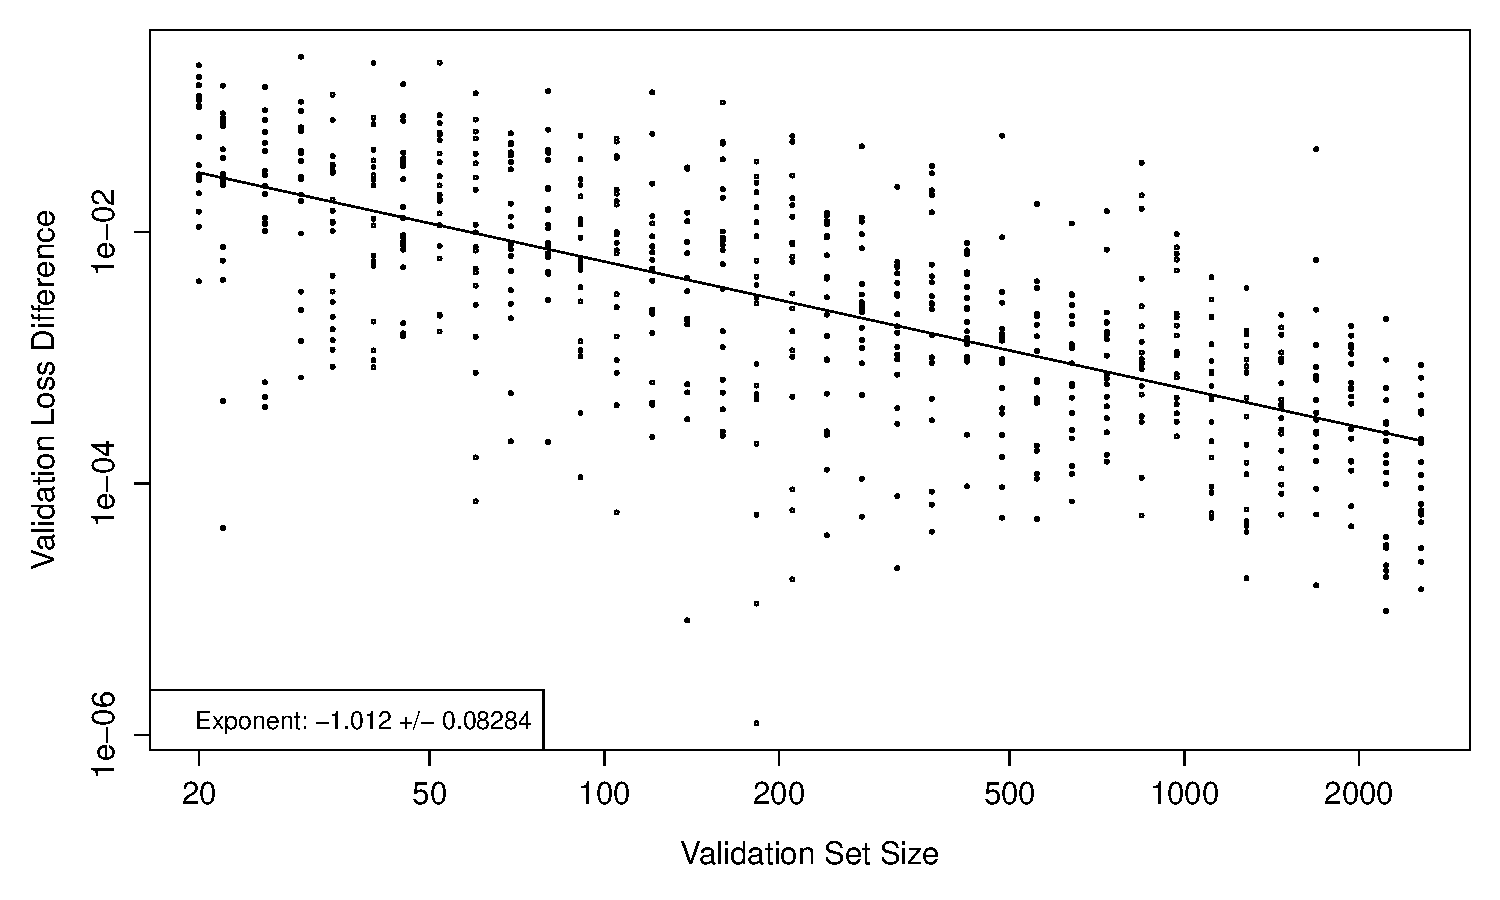
\includegraphics[height=80mm]{../R/figures/validation_size_loss_diff.pdf}
%\includegraphics[height=80mm]{../R/figures/qqplot.pdf}
\end{figure}


\section{Discussion}\label{sec:discussion}

In this paper, we established oracle inequalities for hyperparameter selection using a single training/validation split or $K$-fold cross-validation. The results address the open question regarding model error when many hyperparameters need to be tuned. If the model-estimation procedure is smoothly parameterized by the hyperparameters, then in a non-parametric setting or parametric setting where $p$ grows with $n$, the oracle error is the dominating term in the upper bound. In the parametric setting, the tuning penalty parameter problem contributes an error that is on the same order as the oracle error. 

We then applied our results to penalized regression problems. We showed that the fitted models are Lipschitz in the penalty parameters and get the same relationship between penalty parameters and model error. This suggests that the we should push past the artificial barrier of two penalty parameters and consider combining tens or even hundreds of penalty parameters. For example, Feng and Simon (TBD) fit an un-pooled version of sparse group lasso model with a hundred penalty parameters and significantly decreased the model's generalization error.

A major caveat to our results is that we have assumed that it is possible to find the global minimizer of the validation loss over the penalty parameter space. Unfortunately, this is currently computationally intractable since the validation loss is not convex in the penalty parameters. Better optimization methods need to be developed to solve this problem. Current methods only guarantee finding a local minimizer. More theoretical results are necessary to understand how robust the models are to optimization error.

An interesting direction for future work is to understand the behavior of hyperparameter selection in the hyperparameter space, in contrast to our approach of characterizing model error. For example, bounds on the distance between the selected and oracle penalty parameters
\begin{equation}
\label{penalty_diff}
\left \| \hat{\boldsymbol \lambda} - \tilde{\boldsymbol \lambda} \right \|_2
\end{equation}
can perhaps lend to a more intuitive understanding of hyperparameter selection methods.

\section{The Proof} \label{sec:proofs}

For functions $f$ and $g$ and a dataset $D^{(m)}$ with $m$ samples, we denote the inner product of $f$ and $g$ at covariates $D$ as $\langle f,g \rangle_D = \frac{1}{m} \sum_{x_i \in D} f(x_i) g(x_i) $.

\subsection{Proof for a single training/validation split}
\label{appendix:train_val}

Theorem \ref{thrm:train_val} is a special case of Theorem \ref{thrm:train_val_complicated}, which applies to general model-estimation procedures. The proof is based on the inequality below. Inequalities of this form are often called a ``basic inequality'', since it is derived directly from the definition and the quantity of interest, the difference in the error of the selected model and the oracle model, is bounded by an empirical process term.

\begin{lemma}{Basic inequality}
	\begin{equation}
	\label{thrm:basic_ineq}
	\left \| g^* - \hat{g}^{n_T}(\hat{\boldsymbol{\lambda}}|T) \right \|^2_V 
	- \left \| g^* - \hat{g}^{n_T}(\tilde{\boldsymbol{\lambda}}|T) \right \|^2_V
	\le 
	\left \langle \epsilon, \hat{g}^{n_T}(\tilde{\boldsymbol{\lambda}}|T) - \hat{g}^{n_T}(\hat{\boldsymbol{\lambda}}|T) \right \rangle_V
	\end{equation}
\end{lemma}

\begin{proof}
	By definition,
	\begin{equation}
	\left \| y - \hat{g}^{n_T}(\hat{\boldsymbol{\lambda}}|T) \right \|^2_V \le 
	\left \| y - \hat{g}^{n_T}(\tilde{\boldsymbol{\lambda}}|T) \right \|^2_V
	\end{equation}
\end{proof}

We are therefore interested in bounding the empirical process term in \eqref{thrm:basic_ineq}. A common approach is to use a measure of complexity of the function class. For a single training/validation split, where we treat the training set as fixed, we only need to consider the complexity of the fitted models from the model-selection procedure
\begin{equation}
\mathcal{G}(T)=\left\{ \hat{g}^{(n_T)}(\boldsymbol{\lambda}|T) : \boldsymbol{\lambda} \in \Lambda \right\}
\end{equation}
This model class can be considerably less complex compared to the original function class $\mathcal{G}$, such as the special case in Theorem \ref{thrm:train_val} where we suppose $\mathcal{G}(T)$ is Lipschitz. For this proof, we will use metric entropy as a measure of model class complexity. We recall its definition below.
\begin{definition}
	Let $\mathcal{F}$ be a function class. Let the covering number $N(u, \mathcal{F}, \| \cdot \|)$ be the smallest set of $u$-covers of $\mathcal{F}$ with respect to the norm $\| \cdot \|$. The metric entropy of $\mathcal{F}$ is defined as the log of the covering number:
\begin{equation}
H (u, \mathcal{F}, \| \cdot \| ) = \log N(u, \mathcal{F}, \| \cdot \|)
\end{equation}
\end{definition}

We will bound the empirical process term using the following Lemma, which is a simplification of Corollary 8.3 in \citet{van2000empirical}.

\begin{lemma}
	\label{lemma:cor83}
	Suppose we have dataset $D^{(m)}$ where $\epsilon_1,...,\epsilon_m$ are independent random variables with mean zero and uniformly sub-gaussian with parameter $b > 0$. Suppose
	the model class $\mathcal{F}$ has elements $\sup_{f\in\mathcal{F}}\|f\|_{D^{(m)}}\le R$
	and satisfies
	\[
	\psi(R)\ge\int_{0}^{R}H^{1/2}(u,\mathcal{F},\|\cdot\|_{D^{(m)}})du
	\]
	
	
	There is a constant $a > 0$ dependent only on $b$ such that
	for all $\delta>0$ satisfying
	\[
	\sqrt{m}\delta\ge a(\psi(R)\vee R)
	\]
	
	
	we have 
	\[
	Pr\left(\sup_{f\in\mathcal{F}}\left|\frac{1}{m}\sum_{i=1}^{m}\epsilon_{i}f(x_{i})\right|\ge\delta\right)
	\le 
	a\exp\left(-\frac{m\delta^{2}}{4a^{2}R^{2}}\right)
	\]
	
\end{lemma}

We are now ready to prove the oracle inequality. It uses a standard peeling argument. For readability, we will use the simplified notation $\hat{g}(\hat{\boldsymbol{\lambda}})$ and $\hat{g}(\tilde{\boldsymbol{\lambda}})$.

\begin{theorem}
\label{thrm:train_val_complicated}

Let $\Lambda=[\lambda_{\min},\lambda_{\max}]^{J}$ where $0 < \lambda_{\min} < \lambda_{\max}$. Suppose independent random variables $\epsilon_1, ... \epsilon_n$ have expectation zero and are uniformly sub-Gaussian with parameter $b > 0$.
Suppose there is a function $\psi:\mathbb{R}\mapsto\mathbb{R}$ and constant $r > 0$ such that
\begin{equation}
\label{eq:dudley_bound}
\int_{0}^{R}H^{1/2}(u,\mathcal{G}(T),\|\cdot\|_{V})du\le\psi(R) \quad \forall R>r
\end{equation}
Also, suppose $\psi\left(u\right)/u^{2}$ is non-increasing in $u$ for all $u > r$.
Let $\tilde{\boldsymbol \lambda}$ be defined as in \eqref{eq:tilde_lambda_def}.

Then there is a constant $c>0$ only depending on $b$ such that for all $\delta$ satisfying
\begin{equation}
\label{eq:train_val_delta_condn}
\sqrt{n_V}\delta^{2}
\ge
c \left ( 
\psi(\delta)
\vee 
\delta
\vee
\psi \left (
4\left\Vert g^* - \hat{g}^{(n_T)}( \tilde{\boldsymbol{\lambda}} | T)\right\Vert_{V}^2
\right ) 
\vee
4 \left\Vert g^* - \hat{g}^{(n_T)}( \tilde{\boldsymbol{\lambda}} | T)\right\Vert_{V}^2
\right )
\end{equation}
we have
\begin{eqnarray*}
	Pr\left(
	\left\Vert g^* - \hat{g}^{(n_T)}( \hat{\boldsymbol{\lambda}} | T) \right\Vert _{V}^2 -
	\left\Vert g^* - \hat{g}^{(n_T)}( \tilde{\boldsymbol{\lambda}} | T) \right\Vert _{V}^2
	\ge\delta^2
	\middle | 
	T, X_V
	\right )
	&\le& c\exp\left(-\frac{n_{V}\delta^{4}}{
		c^{2}
		\left\Vert g^* - \hat{g}^{(n_T)}( \tilde{\boldsymbol{\lambda}} | T) \right\Vert _{V}^2
	}\right) \\
	&& +c\exp\left(-\frac{n_{V}\delta^{2}}{c^{2}}\right) \\ 
\end{eqnarray*}
\end{theorem}

\begin{proof}
	The following probabilities are all conditional on $X_V$ and $T$. We leave them out for readability.
	\begin{eqnarray}
		&  & Pr\left(\left\Vert \hat{g}(\hat{\boldsymbol{\lambda}})-g^{*}\right\Vert _{V}^{2}-\left\Vert \hat{g}(\tilde{\boldsymbol{\lambda}})-g^{*}\right\Vert _{V}^{2}\ge\delta^{2}\right) \label{eq:train_val_prob}\\
		& = & \sum_{s=0}^{\infty}Pr\left(2^{2s}\delta^{2}\le\left\Vert \hat{g}(\hat{\boldsymbol{\lambda}})-g^{*}\right\Vert _{V}^{2}-\left\Vert \hat{g}(\tilde{\boldsymbol{\lambda}})-g^{*}\right\Vert _{V}^{2}\le2^{2s+2}\delta^{2}\right) 
		\label{eq:peeled} \\
		&\le&
		Pr\left(2^{2s}\delta^{2}\le2\left\langle \epsilon,\hat{g}(\hat{\boldsymbol{\lambda}})-\hat{g}(\tilde{\boldsymbol{\lambda}})\right\rangle _{V} \wedge
		\left\Vert \hat{g}(\hat{\boldsymbol{\lambda}})-\hat{g}(\tilde{\boldsymbol{\lambda}})\right\Vert_{V}^{2}\le2^{2s+2}\delta^{2}+
		2\left|\left\langle \hat{g}(\tilde{\boldsymbol{\lambda}})-\hat{g}(\hat{\boldsymbol{\lambda}}),\hat{g}(\tilde{\boldsymbol{\lambda}})-g^{*}\right\rangle _{V}\right| \right )
		\label{eq:peel_ineq}
	\end{eqnarray}
	where we applied the basic inequality in the last inequality.
	Each summand in \eqref{eq:peel_ineq} can be bounded by splitting the event into the cases where $2^{2s+2} \delta^2$ is bigger or $2\left|\left\langle \hat{g}(\tilde{\boldsymbol{\lambda}})-\hat{g}(\hat{\boldsymbol{\lambda}}),\hat{g}(\tilde{\boldsymbol{\lambda}})-g^{*}\right\rangle _{V}\right|$ is bigger. Splitting up the probability and applying Cauchy Schwarz gives us the following bound for \eqref{eq:train_val_prob}
	\begin{eqnarray}
	&& Pr\left(
	\sup_{\boldsymbol{\lambda} \in \Lambda: \left\Vert \hat{g}(\cdot|{\boldsymbol{\lambda}})-\hat{g}(\cdot|\tilde{\boldsymbol{\lambda}})\right\Vert _{V}
		\le
		4\left\Vert \hat{g}(\cdot|\tilde{\boldsymbol{\lambda}})-g^{*}\right\Vert _{V}}
	2\left\langle \epsilon,\hat{g}(\cdot|{\boldsymbol{\lambda}})-\hat{g}(\cdot|\tilde{\boldsymbol{\lambda}})\right\rangle _{V}
	\ge 
	\delta^{2}
	\right)
	\label{eq:train_val_1}
	\\
	&& + \sum_{s=0}^{\infty} Pr\left(
	\sup_{\boldsymbol{\lambda} \in \Lambda: \left\Vert \hat{g}(\cdot|{\boldsymbol{\lambda}})-\hat{g}(\cdot|\tilde{\boldsymbol{\lambda}})\right\Vert _{V}
		\le
		2^{s+3/2}\delta}
	2\left\langle \epsilon,\hat{g}(\cdot|{\boldsymbol{\lambda}})-\hat{g}(\cdot|\tilde{\boldsymbol{\lambda}})\right\rangle _{V}
	\ge
	2^{2s} \delta^{2}
	\right)
	\label{eq:train_val_2}
	\end{eqnarray}
	
	We can bound both \eqref{eq:train_val_1} and \eqref{eq:train_val_2} using Lemma \ref{lemma:cor83}. For our choice of $\delta$ in \eqref{eq:train_val_delta_condn},
	there is some constant $a>0$ dependent only on $b$ such that \eqref{eq:train_val_1} is bounded above by
	\[ 
	a\exp\left(-\frac{n_{V}\delta^{4}}{4a^{2}\left(16\left\Vert \hat{g}(\cdot|\tilde{\boldsymbol{\lambda}})-g^{*}\right\Vert _{V}^{2}\right)}\right)
	\]
	In addition, our choice of $\delta$ from \eqref{eq:train_val_delta_condn} and our assumption that $\psi(u)/u^2$ is non-increasing implies that the condition in Lemma \ref{lemma:cor83} is satisfied for all $s=0,1,...,\infty$ simultaneously. Hence for all $s=0,1,...,\infty$, we have
	\[
	Pr\left(
	\sup_{\boldsymbol{\lambda} \in \Lambda: \left\Vert \hat{g}(\cdot|{\boldsymbol{\lambda}})-\hat{g}(\cdot|\tilde{\boldsymbol{\lambda}})\right\Vert _{V}
		\le
		2^{s+3/2}\delta}
	2\left\langle \epsilon,\hat{g}(\cdot|{\boldsymbol{\lambda}})-\hat{g}(\cdot|\tilde{\boldsymbol{\lambda}})\right\rangle _{V}
	\ge
	2^{2s} \delta^{2}
	\right)
	\le 
	a\exp\left(-n_{V}\frac{2^{4s-2}\delta^{4}}{4a^{2}2^{2s+3}\delta^{2}}\right)
	\]
	
	Putting this all together, there is a constant $c$ such that \eqref{eq:train_val_prob} is bounded above by
	\begin{equation}
	c\exp\left(-\frac{n_{V}\delta^{4}}{4 c^{2}\left(16\left\Vert \hat{g}(\cdot|\tilde{\boldsymbol{\lambda}})-g^{*}\right\Vert _{V}^{2}\right)}\right)
	+
	c\exp\left(-\frac{n_{V} \delta^2}{c^{2}}\right)
	\end{equation}
	
\end{proof}

We can apply Theorem \ref{thrm:train_val_complicated} to get Theorem \ref{thrm:train_val}. Before proceeding, we determining the entropy of $\mathcal{G}(T)$ when the functions are Lipschitz in the hyperparameters.

\begin{lemma}
	\label{lemma:covering_cube}
	Let $\Lambda = [\lambda_{\min}, \lambda_{\max}]^J$. Suppose $\mathcal{G}(T)$ is $C$-Lipschitz in $\boldsymbol{\lambda}$ with respect to some norm $\| \cdot \|$.
	Then the entropy of $\mathcal{G}(T)$ with respect to $\| \cdot \|$ is
	\begin{equation}
	H\left(u, \mathcal{G}(T),\|\cdot\|\right) \le
	J \log \left(\frac{4C\left(\lambda_{max}-\lambda_{min}\right)+2u}{u}\right)
	\end{equation}
\end{lemma}
\begin{proof}
	Using a slight variation of the proof for Lemma 2.5 in \citet{van2000empirical}, we can show
	\begin{equation}
	N\left(u,\Lambda,\|\cdot\|_{2}\right) \le \left(\frac{4\left(\lambda_{max}-\lambda_{min}\right)+2u}{u}\right)^{J}
	\end{equation}
	
	Under the Lipschitz assumption, a $\delta$-cover for $\Lambda$
	is a $C\delta$-cover for $\mathcal{G}(T)$. The covering number for $\mathcal{G}(T)$ wrt $\|\cdot\|_{V}$ is bounded by the covering number for $\Lambda$ as follows
	\begin{eqnarray}
	N\left(u,\mathcal{G}(T),\|\cdot\|_{V}\right)
	&\le& N\left(\frac{u}{C},\Lambda,\|\cdot\|_{2}\right)\\
	&\le& \left(\frac{4\left(\lambda_{max}-\lambda_{min}\right)+2u/C}{u/C}\right)^{J}
	\end{eqnarray}
\end{proof}

\paragraph{Theorem \ref{thrm:train_val}}
\begin{proof}
By Lemma \ref{lemma:covering_cube}, we have
\begin{eqnarray*}
	\int_{0}^{R}H^{1/2}(u,\mathcal{G}(T),\|\cdot\|_{V})du 
	&=& \int_{0}^{R} \left ( 
	J \log \left(\frac{4C_\Lambda\left(\lambda_{max}-\lambda_{min}\right)+2u}{u}\right)
	\right )^{1/2}
	du\\
	& \le & J^{1/2}\int_{0}^{R}\left[\log4+\log\left(\frac{8C_\Lambda\left(\lambda_{max}-\lambda_{min}\right)}{u}\right)\right]^{1/2}du\\
	& \le & RJ^{1/2}\left[\int_{0}^{1}\left(\log4+\log\left(\frac{8C_\Lambda\left(\lambda_{max}-\lambda_{min}\right)}{R}\right)+J\log\frac{1}{v}\right)dv\right]^{1/2}\\
	&=& 
	R\left[J \left (
	1+\log \left (32C_\Lambda\left(\lambda_{max}-\lambda_{min}\right)\right)
	+ \log\frac{1}{R} 
	\right )
	\right]^{1/2}
\end{eqnarray*}
where the second inequality follows from a change of variables and the concavity of the square root function. If we restrict $R > n^{-1}$ and $C_\Lambda \ge 32e/(n \lambda_{\max})$, then 
\begin{equation}
\label{eq:train_val_entropy}
\int_{0}^{R}H^{1/2}(u,\mathcal{G}(T),\|\cdot\|_{V})du
\le
\psi (R) \coloneqq 2 R\left ( J \log(C_\Lambda \lambda_{\max}n) \right )^{1/2}
\end{equation}
Applying Theorem \ref{thrm:train_val_complicated}, we get our desired result.
\end{proof}

\subsection{Cross-validation}
We now present the proof for Theorem \ref{thrm:kfold}, which is an application of Theorem 3.5 in \citet{lecue2012oracle}. We reproduce Theorem 3.5 below for convenience. The theorem calculates entropy with respect to the Orlicz norm $\| \cdot \|_{\phi} = \inf \{ C > 0: E[\exp(|f|/C) - 1] \le 1 \}$.

\begin{theorem}
	\label{thrm:mitchell}
	Let $\Lambda = [\lambda_{\min}, \lambda_{\max}]^J$. Let
	$\mathcal{Q} = \{ \| g^* - \hat{g}^{(n_T)}(\boldsymbol{\lambda}|T) \|_2^2 : \boldsymbol{\lambda} \in \Lambda \}$.
	Suppose there is $G > 0$ such that $\sup_{g \in \mathcal{G}} \| g \|_\infty \le G$.
	
	Suppose there is a $d_{\min}$ and a strictly increasing function $\psi$ such that $\psi^{-1}$ is strictly convex, the convex conjugate $\psi^*$ of $\psi^{-1}$ increases, $\psi^*(\infty ) = \infty$ and there exists $r \ge1$ such that $\psi^*(x)/x^r$ is decreasing in $x$ and
	\begin{equation}
	\label{eq:mitchell_dudley_bound}
	\psi(d) \ge \int_0^{\sqrt{d}} H^{1/2}(u, \mathcal{Q}_d, \| \cdot \|_2) du +
	\frac{\log n_V}{\sqrt{n_V}} \int_0^{2G} H(u, \mathcal{Q}_d, \| \cdot \|_\phi) du
	\quad
	\forall d > d_{\min}
	\end{equation}
	where $ \mathcal{Q}_d = \{ Q \in \mathcal{Q}: \| Q \|_2 \le \sqrt{d} \}$.
	
	Suppose that the model-estimation procedure is exchangeable (i.e. any ordering of the same training data produces the same fitted model).
	
	Then for every $a > 0$ and $q > 1$, the following inequality holds
	\begin{eqnarray}
	E_{D^{(n)}} \left \| \bar{g} ( \hat{\boldsymbol \lambda} | {D^{(n)}} ) - g^* \right \|^2 &\le&
	(1+a) \inf_{\boldsymbol{\lambda} \in \Lambda} \left [
	E_{D^{(n_T)}} \left \| \hat{g}^{(n_T)}(\boldsymbol \lambda | D^{(n_T)}) - g^* \right \|^2  
	\right ] \\
	&& + \frac{ac}{q}\left [
	\psi^* \left (\frac{2q^{r}(1+a)}{a\sqrt{n_V}} \right ) \vee d_{\min}
	\right ]
	\end{eqnarray}
\end{theorem}

In order to apply Theorem \ref{thrm:mitchell}, we need to determine the entropy of the loss functions with respect to the Orlicz norm.

\paragraph{Theorem \ref{thrm:kfold}}
\begin{proof}
	First we determine $\psi$ in \eqref{eq:mitchell_dudley_bound}. Note that because $\|\cdot\|_\phi \le 2\|\cdot \|_\infty $ and $\| \cdot \|_2 \le \| \cdot \|_\infty$, then both $H(2u,\mathcal{Q}_{d}(T),\|\cdot\|_{\phi})$ and $H(u,\mathcal{Q}_{d}(T),\|\cdot\|_2)$ are bounded by 
	$H(u,\mathcal{Q}_{d}(T),\|\cdot\|_{\infty})$.
	By Lemma \ref{lemma:covering_cube}, we know
	\begin{equation}
	H(u,\mathcal{Q}_{d}(T),\|\cdot\|_{\infty}) \le J \log\left [
	\frac{16GC\lambda_{\max} + 2u}{u}
	\right ]
	\end{equation}
	Hence we can let
	\begin{equation}
	\psi(d) \coloneqq
	\sqrt{d}K_{n,1}
	+
	\frac{K_{n,2}}{\sqrt{n_V}} 
	\end{equation}
	for $K_{n,1} = \left[J\left(1+\log\left(128\sqrt{n_V} GC\lambda_{max}  \right)\right)\right]^{1/2}$ and $K_{n,2} = \log n_V 2GJ\left(1+\log\left(128GC\lambda_{max}\right)\right)$. $\psi(d)$ is a valid upper bound in \eqref{eq:mitchell_dudley_bound}  for all $d > n_V^{-1}$.
	
	We can show that the convex conjugate of $\psi^{-1}$ is
	\begin{equation}
	\label{eq:convex_conjugate}
	\psi^*(z) = \frac{z^2 K_{n,1}^2}{4} + \frac{z K_{n,2}}{\sqrt{n_V}}
	\end{equation}	
	
	Plugging in \eqref{eq:convex_conjugate} into Theorem \ref{thrm:mitchell} gives us the result in Theorem \ref{thrm:kfold}.
\end{proof}

\subsection{Penalized regression for additive models}

We now show that penalized regression problems for additive models satisfies the Lipschitz condition.

\paragraph{Lemma \ref{lemma:param_add}}
\begin{proof}
By the gradient optimality conditions, we have for all $j=1:J$ 
\begin{equation}
\label{eq:grad_opt}
\left.\nabla_{\theta^{(j)}} \left [
\frac{1}{2}\left\Vert y-g(\boldsymbol{\theta})\right\Vert _{T}^{2}+\lambda_{j}P_{j}(\boldsymbol{\theta}^{(j)})
\right ]
\right|_{\boldsymbol{\theta}=\hat{\boldsymbol{\theta}}(\lambda)}=0
\end{equation}

Now we implicitly differentiate with respect to $\boldsymbol{\lambda}$ 
\begin{equation}
\label{eq:implicit_diff}
\nabla_{\lambda}\left\{ \left.\nabla_{\theta^{(j)}}
\left [
\frac{1}{2}\left\Vert y-g(\boldsymbol{\theta})\right\Vert _{T}^{2}+\lambda_{j}P_{j}(\boldsymbol{\theta}^{(j)})
\right ]
\right|_{\boldsymbol{\theta}=\hat{\boldsymbol{\theta}}(\boldsymbol{\lambda})}\right\} =0
\end{equation}

Define the following matrices 
\begin{eqnarray*}
	S = \left.\nabla_{\theta}\left [
	\frac{1}{2}\left\Vert y-g(\boldsymbol{\theta})\right\Vert _{T}^{2}
	\right ]
	\right|_{\boldsymbol{\theta}=\hat{\boldsymbol{\theta}}(\lambda | T)}
	\end{eqnarray*}
	
	\[
	D=\left.diag\left(\left\{ \nabla_{\boldsymbol{\theta}^{(j)}}^{2}\lambda_{j}P_{j}(\boldsymbol{\theta}^{(j)})\right\} _{j=1}^{J}\right)\right|_{\boldsymbol{\theta}=\hat{\boldsymbol{\theta}}(\lambda|T)}
	\]
	
	
	\[
	M: \text{column } M_j = \left. \nabla_{\theta}P_{j}(\boldsymbol{\theta}^{(j)})
	\right|_{\boldsymbol{\theta}=\hat{\boldsymbol{\theta}}(\lambda|T)}
	\]
	From the product rule and chain rule, we can then write the system of equations in \eqref{eq:implicit_diff} as
	\begin{equation}
	\label{eq:param_matrix}
	\left(\begin{array}{cccc}
	\nabla_{\lambda}\hat{\boldsymbol{\theta}}_{1}(\boldsymbol{\lambda}) & \nabla_{\lambda}\hat{\boldsymbol{\theta}}_{2}(\boldsymbol{\lambda}) & ... & \nabla_{\lambda}\hat{\boldsymbol{\theta}}_{p}(\boldsymbol{\lambda})\end{array}\right)=-M^{\top}\left(S+D\right)^{-1}
	\end{equation}
	We now bound each column in $M$. From the \eqref{eq:grad_opt} and Cauchy Schwarz, we have 
	\begin{eqnarray*}
		\left\Vert \left.\nabla_{\theta^{(j)}}P_{j}(\boldsymbol{\theta}^{(j)})\right|_{\boldsymbol{\theta}=\hat{\boldsymbol{\theta}}(\lambda)}\right\Vert  & \le & \frac{1}{\lambda_{min}\sqrt{n_{T}}}\left\Vert y-g(\cdot|\hat{\boldsymbol{\theta}}(\boldsymbol{\lambda}))\right\Vert _{T}\sqrt{\sum_{i=1}^{n_{T}}\left\Vert \nabla_{\theta^{(j)}}g_{j}(x_{i}|\boldsymbol{\theta}^{(j)})\right\Vert _{2}^{2}}		
	\end{eqnarray*}
	The norm of the gradients of $g_j$ can be bounded since $g_j$ is Lipschitz. Also, by definition of $\hat{\boldsymbol{\theta}}(\boldsymbol{\lambda})$, we have
	\begin{eqnarray}
	\frac{1}{2}\left\Vert y-g(\cdot|\hat{\boldsymbol{\theta}}(\boldsymbol{\lambda}))\right\Vert _{T}^{2}+\sum_{j=1}^{J}\lambda_{j}P_{j}\left(\hat{\boldsymbol{\theta}}^{(j)}(\boldsymbol{\lambda})\right) & \le & \frac{1}{2}\left\Vert y-g(\cdot|\boldsymbol{\theta}^{*})\right\Vert _{T}^{2}+\sum_{j=1}^{J}\lambda_{j}P_{j}(\boldsymbol{\theta}^{(j),*})\\
	& \le & C_{\theta^{*},\Lambda}
	\end{eqnarray}
	
	Hence for all $j=1,...,J$
	\begin{eqnarray*}
		\left\Vert \left.\nabla_{\theta^{(j)}}P_{j}(\boldsymbol{\theta}^{(j)})\right|_{\boldsymbol{\theta}=\hat{\boldsymbol{\theta}}(\lambda)}\right\Vert  & \le & \frac{L}{\lambda_{min}}\sqrt{2C_{\theta^{*},\Lambda}}
	\end{eqnarray*}

	Now we bound the norm of $\nabla_\lambda \hat{\boldsymbol{\theta}}(\boldsymbol{\lambda})$. From \eqref{eq:param_matrix}, we have for all $j=1,...,J$
	\begin{eqnarray*}
		\|\nabla_{\lambda}\hat{\boldsymbol{\theta}}_{i}(\boldsymbol{\lambda})\| & = & \|M^{\top}\left(S+D\right)^{-1}e_{k}\|\\
		& \le & \sum_{j=1}^{J}\left\Vert \left.\nabla_{\theta^{(j)}}P_{j}(\boldsymbol{\theta}^{(j)})\right|_{\boldsymbol{\theta}=\hat{\boldsymbol{\theta}}(\lambda)}\right\Vert _{2}\left\Vert \left(S+D\right)^{-1}\right\Vert _{2}\\
		& \le & J\left(\frac{L}{\lambda_{min}}\sqrt{2C_{\theta^{*},\Lambda}}\right)\frac{1}{m}
	\end{eqnarray*}
	where the last line follows from the fact that $(S + D)^-1 \succeq m^{-1}I$. Since the norm of the gradient is bounded, $\hat{\boldsymbol{\theta}}(\boldsymbol{\lambda})$ must be Lipschitz
	\begin{equation}
	\left\Vert \hat{\boldsymbol{\theta}}(\boldsymbol{\lambda})-\hat{\boldsymbol{\theta}}(\boldsymbol{\lambda}')\right\Vert _{2}\le\frac{LJ^{3/2}\sqrt{2C_{\theta^{*},\Lambda}}}{m\lambda_{min}}\|\boldsymbol{\lambda}-\boldsymbol{\lambda}'\|_{2}
	\end{equation}
	Finally the result \eqref{eq:param_add_lipschitz} clearly follows since $g_j(\boldsymbol{\theta})$ are Lipschitz in $\boldsymbol{\theta}$ with respect to $\| \cdot \|_\infty$.
\end{proof}

\paragraph{Lemma \ref{lemma:nonsmooth}}

\begin{proof}
	Consider any $\boldsymbol{\lambda^{(1)}},\boldsymbol{\lambda^{(2)}}\in\Lambda_{smooth}$. 
	
	From Condition \ref{condn:nonsmooth1}, every point $\boldsymbol{\lambda} \in \Lambda_{smooth}$ is the center of a ball $B(\boldsymbol{\lambda})$ with nonzero radius where the differentiable space within $B(\boldsymbol{\lambda})$ is constant.
	Hence by Condition \ref{condn:nonsmooth2}, it can be shown that there must exist a countable
	set of points $\bar{\boldsymbol{\ell}} 
	%=\cup_{i=1}^{\infty}\boldsymbol{\ell}^{(i)}
	\subset\mathcal{L}(\boldsymbol{\lambda^{(1)}},\boldsymbol{\lambda^{(2)}})$ where $\boldsymbol{\lambda}^{(1)}, \boldsymbol{\lambda}^{(2)} \in \bar{\boldsymbol{\ell}}$
	such that the union of their differentiable neighborhoods cover  $\mathcal{L}(\boldsymbol{\lambda^{(1)}},\boldsymbol{\lambda^{(2)}})$ entirely:
	\[
	%\mu_{1}\left(\cup_{i=1}^{\infty}B(\boldsymbol{\ell}^{(i)})
	\mu_{1}\left(\cup_{\ell \in \bar{\boldsymbol{\ell}}}B(\boldsymbol{\ell})
	\cap\mathcal{L}\left(\boldsymbol{\lambda^{(1)}},\boldsymbol{\lambda^{(2)}}\right)\right)=\left\Vert \mathcal{L}\left(\boldsymbol{\lambda^{(1)}},\boldsymbol{\lambda^{(2)}}\right)\right\Vert _{2}
	\]
	where $\mu_{1}$ is the Lebesgue measure over  $\mathcal{L}(\boldsymbol{\lambda^{(1)}},\boldsymbol{\lambda^{(2)}})$.
	
	Consider the intersections of boundaries of the differentiable neighborhoods with the line segment:
	\[
	P=
	\left ( 
	\cup_{\ell \in \bar{\boldsymbol{\ell}}}
	\mbox{Bd}B\left(\boldsymbol{\ell}\right)
	\right )
	\cap\mathcal{L}(\boldsymbol{\lambda^{(1)}},\boldsymbol{\lambda^{(2)}})
	\]
	Every point $p\in P$ can be expressed as $\alpha_{p}\boldsymbol{\lambda^{(1)}}+(1-\alpha_{p})\boldsymbol{\lambda^{(2)}}$
	for some $\alpha_{p}\in[0,1]$. So points in $P$ can ordered by increasing $\alpha_{p}$ to get the sequence $\boldsymbol{p}^{(1)}, \boldsymbol{p}^{(2)}, ... $.
	By Condition \ref{condn:nonsmooth1}, the differentiable space of the training criterion
	is also constant over $\mathcal{L}\left(\boldsymbol{p}^{(i)},\boldsymbol{p}^{(i+1)}\right)$ since each of these sub-segments are a subset of $B(\boldsymbol{\ell})$ for some $\boldsymbol{\ell} \in \bar{\boldsymbol{\ell}}$. 
	
	Let the differentiable
	space over the interior of line segment $\mathcal{L}\left(\boldsymbol{p^{(i)},p^{(i+1)}}\right)$
	be denoted $\Omega_{i}$. 
	By Condition \ref{condn:nonsmooth1}, the differentiable space is also a local optimality
	space. Let $U^{(i)}$ be an orthonormal basis of $\Omega_{i}$. For
	each $i$, we can express $\hat{\boldsymbol{\theta}}(\boldsymbol{\lambda} | T)$ for
	all $\boldsymbol{\lambda}\in\mbox{Int}\left\{ \mathcal{L}\left(\boldsymbol{p^{(i)},p^{(i+1)}}\right)\right\} $
	as
	\[
	\hat{\boldsymbol{\theta}}(\boldsymbol{\lambda} | T)=U^{(i)}\hat{\boldsymbol{\beta}}(\boldsymbol{\lambda} | T)
	\]
	\[
	\hat{\boldsymbol{\beta}}(\boldsymbol{\lambda} | T)=\arg\min_{\beta}L_{T}(U^{(i)}\boldsymbol{\beta},\boldsymbol{\lambda})
	\]
	Apply Lemma \ref{lemma:param_add} with $\Lambda= \mathcal{L}\left(\boldsymbol{p^{(i)},p^{(i+1)}}\right)$, and modify the proofs to take directional derivatives
	along the columns of $U^{(i)}$ instead. Then there is a constant
	constant $c>0$ independent of $i$ such that for all $i=1,2...$,
	such that
	\[
	\left\Vert 
	\boldsymbol{\hat{\beta}}(\boldsymbol{p}^{(i)} | T)
	-\boldsymbol{\hat{\beta}}(\boldsymbol{p}^{(i)} | T)
	\right\Vert _{2}
	\le 
	c\|\boldsymbol{p}^{(i)}-\boldsymbol{p}^{(i+1)}\|_{2}
	\]
	
	
	Finally, we can sum these inequalities. By the triangle inequality,
	\begin{eqnarray*}
		\left\Vert 
		\hat{\theta}(\boldsymbol{\lambda}^{(1)} |T)
		- \hat{\theta}(\boldsymbol{\lambda}^{(2)} |T)
		\right\Vert _{2} 
		& \le & \sum_{i=1}^{\infty}\|\boldsymbol{\hat{\theta}}_{p^{(i)}}-\boldsymbol{\hat{\theta}}_{p^{(i+1)}}\|_{2}\\
		& \le & \sum_{i=1}^{\infty}
		c\|\boldsymbol{p}^{(i)}-\boldsymbol{p}^{(i+1)}\|_{2}\\
		& = & c\|\boldsymbol{\lambda}^{(1)}-\boldsymbol{\lambda}^{(2)}\|_{2}
	\end{eqnarray*}
\end{proof}

\paragraph{Lemma \ref{lemma:nonparam_smooth}}

\begin{proof}
	Let $H_{0} = \left \{
	j:\left\Vert \hat{g}_{j}(\boldsymbol{\lambda}^{(2)}|T)-\hat{g}_{j}(\boldsymbol{\lambda}^{(1)}|T)\right\Vert _{D^{(n)}} \ne 0 \forall j = 1,...,J
	\right \}$.
	For all $j \in H_0$, let 
	\[
	h_{j}=
	\frac{\hat{g}_{j}(\boldsymbol{\lambda}^{(2)}|T)-\hat{g}_{j}(\boldsymbol{\lambda}^{(1)}|T)}{\left\Vert \hat{g}_{j}(\boldsymbol{\lambda}^{(2)}|T)-\hat{g}_{j}(\boldsymbol{\lambda}^{(1)}|T)\right\Vert _{D^{(n)}}}
	\]
	For notational convenience, let $\hat{g}_{1,j} = \hat{g}_{j}(\boldsymbol{\lambda}^{(1)}|T)$. Consider the optimization problem
	\begin{equation}
	\hat{\boldsymbol{m}}(\boldsymbol{\lambda})=\left\{ \hat{m}_{j}(\boldsymbol{\lambda})\right\} _{j\in H_0}
	=\argmin_{m_{j} \in \mathbb{R}: j\in H_0}
	\frac{1}{2}
	\left \|y-\sum_{j=1}^{J}\left(\hat{g}_{1,j}+m_{j}h_{j}\right) \right \|_{T}^{2}
	+\sum_{j=1}^{J}\lambda_{j}
	P_{j} \left (\hat{g}_{1,j}+m_{j}h_{j} \right )
	\end{equation}
	By the gradient optimality conditions, we have
	\begin{equation}
		\nabla_{m} \left .
		\left[\frac{1}{2}\|y-\sum_{j=1}^{J}\left(\hat{g}_{1,j}+m_{j}h_{j}\right)\|_{T}^{2}+\sum_{j=1}^{J}\lambda_{j}P_{j}(\hat{g}_{1,j}+m_{j}h_{j})\right] \right |_{m=\hat{m}(\lambda)}
		= 0
		\label{eq:nonparam_grad_opt}
	\end{equation}
	Implicit differentiation with respect to $\boldsymbol{\lambda}$ gives us
	\begin{equation}
		\nabla_\lambda 
		\nabla_m
		\left . \left[
		\frac{1}{2}\|y-\sum_{j=1}^{J}\left(\hat{g}_{1,j}+m_{j}h_{j}\right)\|_{T}^{2}+\sum_{j=1}^{J}\lambda_{j}P_{j}(\hat{g}_{1,j}+m_{j}h_{j})\right] \right |_{m=\hat{m}(\lambda)}
		= 0
		\label{eq:nonparam_imp_diff}
	\end{equation}
	Define the following matrices
	\[
	S:S_{ij}=\langle h_{j},h_{j}\rangle_{T}
	\]
	\[
	D_{1}=diag\left(
	\left \{
	\left.\lambda_{j}\frac{\partial^{2}}{\partial m_{j}^{2}}P_{j}(\hat{g}_{1,j}+m_{j}h_{j})\right|_{m=\hat{m}(\lambda)}
	\right \}_{j=1}^J
	\right)
	\]
	
	
	\[
	D_{2}=diag\left(\left \{ \left.
	\frac{\partial}{\partial m_{j}}P_{j}(\hat{g}_{1,j}+m_{j}h_{j})\right|_{m=\hat{m}(\lambda)}
	\right \}_{j=1}^J
	\right)
	\]
	
	
	\[
	M:\mbox{ column }M_{j}=\nabla_{\lambda}\hat{m}_{j}(\lambda) \quad \forall j=1,...,J
	\]
	
	
	The system of equations from \eqref{eq:nonparam_imp_diff} can be written as  $M=D_{2}\left(S+D_{1}\right)^{-1}$.
	
	Now we bound each element in $D_2$. From \eqref{eq:nonparam_grad_opt} and Cauchy Schwarz, we have for all $k=1,...,J$
	\begin{equation}
		\left|\frac{\partial}{\partial m_{k}}P_{k}(\hat{g}_{1,k}+m_{k}h_{k})\right|_{m=\hat{m}(\lambda)}
		\le 
		\frac{1}{\lambda_{min}}
		\left\Vert y-\sum_{j=1}^{J}\left(\hat{g}_{1,j}+\hat{m}_{j}(\boldsymbol{\lambda})h_{j}\right)
		\right\Vert _{T}\|h_{k}\|_{T}
	\end{equation}
	We note that $\|h_{k}\|_{T} \le \sqrt{\frac{n_{D}}{n_{T}}}$. Also, by definition of $\hat{m}(\boldsymbol{\lambda})$,
	\begin{eqnarray*}
	\frac{1}{2}\left\Vert y-\sum_{j=1}^{J}\left(\hat{g}_{1,j}+\hat{m}_{j}(\boldsymbol{\lambda})h_{j}\right)\right\Vert _{T}^{2}+\sum_{j=1}^{J}\lambda_{j}P_{j}(\hat{g}_{1,j})
	& \le & \frac{1}{2}\left\Vert y-\sum_{j=1}^{J}\hat{g}_{1,j}\right\Vert _{T}^{2}+\sum_{j=1}^{J}\lambda_{j}P_{j}(\hat{g}_{1,j})\\
	& \le & C_{\Lambda}^* + J\lambda_{max}\max_{j=1:J}P_{j}(\hat{g}_{1,j})
	\end{eqnarray*}
	Hence every diagonal element in $D_2$ is bounded above by
	\begin{equation}
	\frac{1}{\lambda_{min}}
	\sqrt{2C_{\Lambda}^* \frac{n_{D}}{n_{T}}\left(1+\frac{J\lambda_{max}}{\lambda_{min}}\right)}
	\end{equation}
	
	
	Now we can bound the norm of the gradient $\boldsymbol{\hat{m}}_k(\boldsymbol{\lambda})$ for $k \in H_0$
	\begin{eqnarray}
	\|\nabla_{\lambda}\hat{m}_{k}(\boldsymbol{\lambda})\|
	& = & \left\Vert D_{2}\left(S+D_{1}\right)^{-1}e_{k}\right\Vert \\
	& \le & \frac{1}{\lambda_{min}}
		\sqrt{2C_{\Lambda}^*
		\frac{n_{D}}{n_{T}}\left(1+\frac{J\lambda_{max}}{\lambda_{min}}\right)}\left\Vert \left(S+D_{1}\right)^{-1}e_{k}\right\Vert \\
	\end{eqnarray}
	By the assumption in \eqref{eq:gateuax}, $e_{k}^\top \left(S+D_{1}\right) e_{k} \ge m$.
	
	By the mean value theorem and Cauchy Schwarz, we have
	\begin{equation}
		\left|\hat{m}_{j}(\boldsymbol{\lambda}^{(2)})-\hat{m}_{j}(\boldsymbol{\lambda}^{(1)})\right| 
		\le \left\Vert \boldsymbol{\lambda}^{(2)}-\boldsymbol{\lambda}^{(1)}\right\Vert \frac{1}{d\lambda_{min}}\sqrt{2C^*_\Lambda \frac{n_{D}}{n_{T}}\left(1+\frac{J\lambda_{max}}{\lambda_{min}}\right)}
	\end{equation}
	Since $
	\left|
	\hat{m}_{j}(\boldsymbol{\lambda}^{(2)})-\hat{m}_{j}(\boldsymbol{\lambda}^{(1)})
	\right|  =
	\left \| 
	\hat{g}_{j}(\boldsymbol{\lambda}^{(2)}|T)-\hat{g}_{j}(\boldsymbol{\lambda}^{(1)}|T)
	\right  \|_{D^{(n)}}
	$, the result in \eqref{eq:nonparam_lipshitz_thrm} follows.
	
	
\end{proof}


\bigskip

\bibliographystyle{agsm}
\bibliography{multi-penalties-theory}

\end{document}
